%% -*- coding: utf-8 -*-
\documentclass{article}
% Outline for statistics tutorial
% Hal Canaray and Cory Quammen
\usepackage{graphicx}
\usepackage{utfsymb}
\usepackage{hyperref}
\begin{document}

\begin{center}
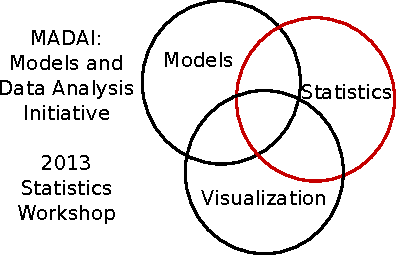
\includegraphics{figures/MADAI_2013_Stats_Workshop.pdf}\\
\url{http://madai.us/}
\end{center}

\section{Statistics background}

\subsection{Basic concepts}

We have a model and we're trying to find parameters for it that best
explain some observed phenomena.

\begin{itemize}

\item \textbf{Model} — a conceptual model of a physical process.  It exists as
  a procedure that takes in parameters and returns a set of
  outputs and potentially uncertainty about those outputs. FIXME Examples
 
\item \textbf{Observables} — a set of field measurements that can be compared
  against a model's outputs. FIXME Examples

\item \textbf{Output Space} — The set of all possible outputs of the model,
  which are intended to be compared to observables.

\item \textbf{Model Outputs} — a point in output space, or a point in output
  space together wuith uncertainty.

\item \textbf{Model Parameters} — any of the modifiable inputs to the
  model. FIXME Examples

\item \textbf{Parameter Space} — the set of all possible values for each of the
  parameters

\item \textbf{Ground Truth} — a point in parameter space that represents how
  the physical process actually works.

\item \textbf{Likelihood} — Given a model and set of observables, this is the
  probability that a given set of parameter values is the ground truth.

\item \textbf{Prior Likelihood} — FIXME
\end{itemize}

\newpage

\[ P = \textrm{parameter space} ⊂ ℝ^p \qquad
 T = \textrm{output space} ⊂ ℝ^t \]
\[ M: P → T  = \textrm{a model} \]
\[ Y_f = \textrm{distribution of field measurements} ⊂ T \]
\[ E[·] = \textrm{expectation value} \qquad Σ[·] = \textrm{covariance matrix} \]
\[ ℒ_{M,Y_f}: P → ℝ^+. \qquad
 ℒ_{M,Y_f}(x) = \textrm{likelihood of $x$, given $M$ and $Y_f$} \]
\[
ℒ_M(x) ∝ \textrm{exp}\left({-\frac{1}{2}\big(E[M(x)]-E[Y_f]\big)^T
     \big(Σ[M(x)]+Σ[Y_f]\big)^{-1} \big(E[M(x)]-E[Y_f]\big)}\right)
\]

\begin{center}
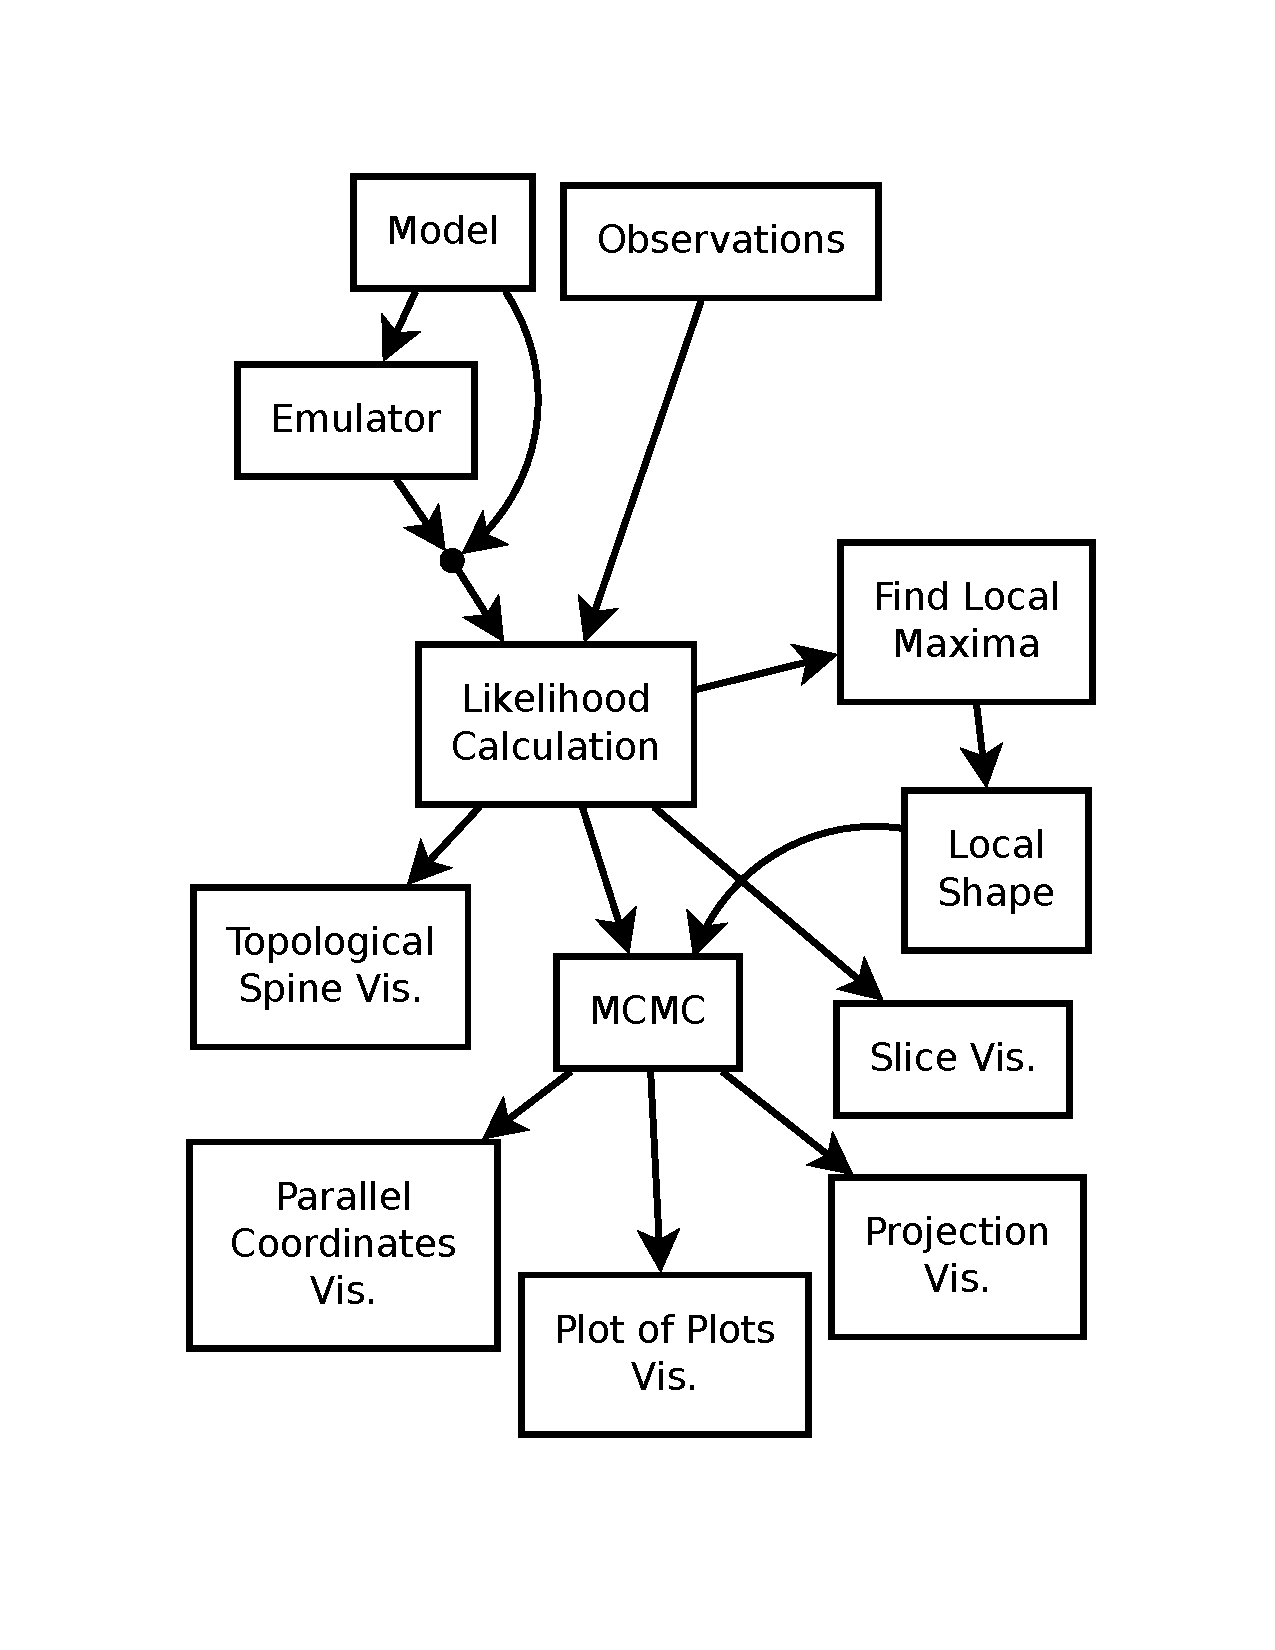
\includegraphics[width=3in]{figures/MADAI_Stats_and_Vis.pdf}
\end{center}


\section{ So you want to effectivly explore the parameter space of your model?}

This HOWTO is intended to be used by someone just about to start the
process

\begin{enumerate}

\item Step one: effectivly parametrarize your model. Choose parameters
  that vary in the same scale (this makes the numerical process
  easier). If a parameter $Q$ varies from 1.0e-4 to 1.0e4, consider
  defining $q := \ln(Q/min)/\ln(max/min)$.

\item Decide which model outputs you want to use. These should be
  numbers which can be readily compared to your experimental /
  observational data.

\item Choose a number of samples. One rule of thumb is that you need
  more than $10×$ the number of parameters. This is constrained by
  your processing power and the complexity of your model.  The more
  samples you choose, the better your emulator will be.

\item Generate a Latin hypercube sample of the parameter space. 

\item Evaluate your model at the sample points.

\item Assemble the sample points together with the model outputs into
  a file suiatable for input into the MADAI Gaussian Process Model
  Emulator.  See the manpage of the emulator for more information.

\item Use the “Estimate Hyperparameters” function of the emulator to
  generate a Gaussian process model of your model. Check that it works
  well, then tweek the settings on the Hyperparameters Estimation. Ask
  for help if it doesn’t work well.

\item Pass the GP model state into the Distribution Sampling tools.

\end{enumerate}

\subsubsection{Probability and statistics review}

Touch on terms.

Probability, expectation, distribution, joint distribution, variance,
covariance

\subsubsection{Joint implausbility and log-likelihood}

\section{Gaussian process emulator}

\subsection{Background}

See Chris Coleman-Smith's presentation at the June 2012 MADAI meeting on this

\begin{itemize}

\item What it does?

\item Why use it instead of interpolation?

\item How to use it?

\end{itemize}

{\raggedleft
\textsf{This section taken from MADAI/MADAIEmulator.git::README}

}

A project to implement scalar Gaussian process regression with a
variety of covariance functions with an optional (up to 3rd order)
linear regression prior mean. Maximum likelihood hyper-parameters can
be estimated to parametrize a given set of training data. For a given
model (estimated hyperparams and training data set) the posterior mean
and variance can be sampled at arbitrary locations in the parameter
space.

The model parameter space can take any dimension (within limits of the
optimizer), output must be scalar.

Gaussian Process regression is a supervised learning method, a
representative set of samples of a model's output can be used to build
a predictive distribution for the output at untried locations in the
models parameter space. This code base has been developed to apply
this process to the output of complex computer codes.

Suppose we have a model $M$ which produces a single scalar output as a
function of some set of input parameters $x∈P$. A design is a set of
points $D = \{x_1, …, x_n\}⊂P$ in the $x$ space at which we will evaluate
the model. A set of training outputs $Y_t = \{M(x_1), …, M(x_n)\} ⊂ ℝ$ is
produced by evaluating the model at each location in $D$. The sets $D$ and
$Y_t$ are then sufficient to 'train' a GP regression model or Emulator
to produce predictions at some new locations $x^*$.

The training process conditions a Gaussian Process prior on 
$(D,Y_t,)$ such that functions drawn from the ensuing posterior will
always pass through the training locations. A Gaussian Process (GP) is
a stochastic process for which any finite set of samples have a multi
variate normal distribution. In essence we force the Gaussian Process
to always generate functions which interpolate our data set.

The GP is specified in terms of a prior mean, usually chosen to be
zero or given by a simple regression model of the training data, and a
covariance function over the parameter space. The covariance function $C_Θ$
specifies the correlation between pairs of parameter values $u, v ∈
P$. A power exponential form, with a nugget, is the default.  
\[
\textrm{Squared-Exponential}_Θ(u, v)
 = θ_0 \textrm{~exp}\left({-\frac{1}{2} \sum_{i=0}^{p-1} \frac{(u_i - v_i)^2}{(θ_{2+i})^2}}\right) + θ_1. \]
for $Θ = (θ_0, θ_1, θ_2, …, θ_{p+1})$.

Other examples of covariance functions are: $C_Θ = \textrm{Matérn}_{3/2,Θ}$ or 
$C_Θ = \textrm{Matérn}_{5/2,Θ}$ with $Θ = ({θ_0}, {θ_1}, {θ_2})$:
\[
\textrm{Matérn}_{3/2,Θ}(u,v) = 
{θ_0} \left({ 1 + e^{- θ_2} \sqrt{3} ‖u-v‖ }\right) 
\exp \left({ - e^{- θ_2} \sqrt{3} ‖u-v‖ }\right) + {θ_1}
\]
\[
\textrm{Matérn}_{5/2,Θ}(u,v) = 
{θ_0} \left({ 1 + \sqrt{5}  \dfrac{ ‖u-v‖}{e^{θ_2}}
 + \dfrac{5}{3} \left({\dfrac{‖u-v‖}{e^{θ_2}}}\right)^2  }\right) 
\exp \left({ - \sqrt{5}\dfrac{ ‖u-v‖}{e^{θ_2}} }\right) + {θ_1} \]

\begin{center}
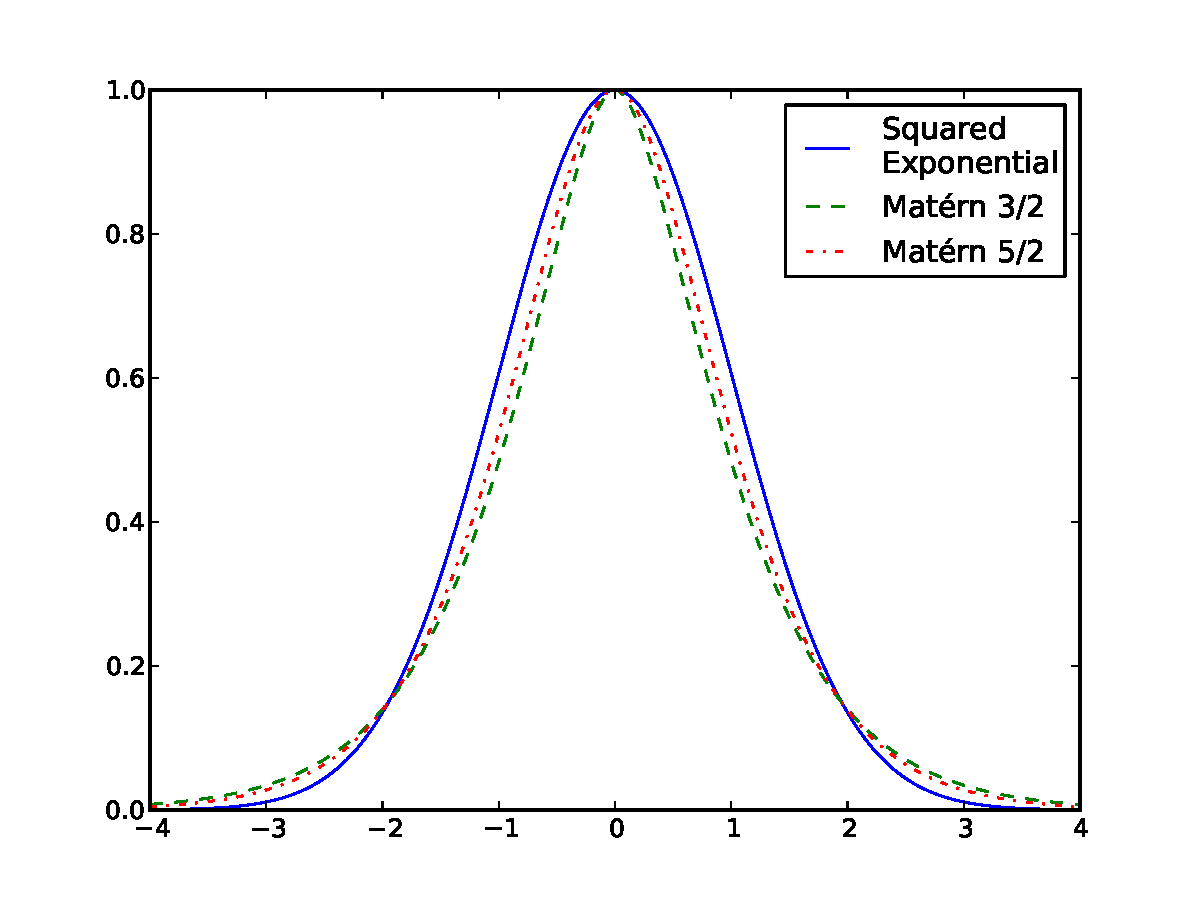
\includegraphics[width=3in]{figures/kernel_functions.pdf}
\end{center}

The covariance function itself is controlled by a set of
hyper-parameters $θ_i$, these act as characteristic length scales in
the parameter space and are a-priori unknown. The training process
consists of estimating the 'best set of length scales for the given
model data set. This estimation process is done through numerical
maximization of the posterior hyper parameter likelihood, a fully
Bayesian treatment is also possible.

Once the GP has been conditioned, and a best set of hyper parameters
$Θ$ has been obtained, we have a posterior predictive distribution
for the model output at a new location $x^*$:

\[P(M(x^*) | Y_t, D, Θ)
	= \textrm{Multivariate-Normal}(\textrm{mean}(x^*), \textrm{cov}(x^*)), \]

where the posterior mean and covariance are (for a zero prior mean)

\[ \textrm{mean}(x^*) = C_Θ(x^*,D)^T  C_Θ(D,D)^{-1} Y_t \]
\[ \textrm{cov}(x^*) = C_Θ(x^*,x^*) - C_Θ(x^*,D)^T C_Θ(D,D)^{-1} C(x^*,D). \]

Here $C_Θ(D,D)$ represents the matrix formed by evaluating the
covariance function $C_Θ$ at each pair of locations in $D$, the vector
$C_Θ(x^*,D)$ is the correlation between each location in the design
set and the new point.

\[ \textrm{matrix } C_Θ(D_Θ,D_Θ)_{i,j} = C_Θ(x_i,x_j)
	 \qquad \textrm{for } x_i,x_j ∈ D \]
\[ \textrm{vector } C_Θ(x^*,D_Θ)_{i} = C_Θ(x^*,x_i)
	 \qquad \textrm{for } x_i ∈ D, x^* ∈ P \]

These equations have a relatively straightforward interpretation. The
prior mean (0) is modified by the covariance structure deduced from
the data \\
$C_Θ(x^*,D)^T C_Θ(D,D)^{-1} Y_t$, \\
at $x^* = x_i$ where $x_i$ is in $D$,
we can see that $m(x_i) = 0$.

\[ C_Θ(x_i,D)^T C_Θ(D,D)^{-1} Y_t = (Y_t)_i \]

 The prior covariance at $x^*, C_Θ(x^*,x^*)$ is
somewhat reduced by the training set $C_Θ(x^*,D)^t C_Θ(D,D)^{-1}
C_Θ(x^*,D)$ and again at $x^*=x_i$ for $x_i∈D$ we reduce to $\textrm{cov}(x_i) =
0$. As such we have constructed an interpolating function.

It is important to note that unlike some other data
interpolation/extrapolation methods we end up with a probability
distribution for the value of our model at an untried location, as it
is normal the mean and covariance are sufficient to describe the
distribution. These can be obtained by the \texttt{emulate\_at\_point} or
\texttt{emulate\_at\_list} functions.

It is straightforward to draw samples from the predictive
distribution, although care must be taken to expand the above
equations correctly for a set of m observation locations
$X^* = {x^*_1, ... x^*_m}$.

For more information see the documentation, the website
\url{http://www.gaussianprocess.org/} and the invaluable book
\emph{Gaussian Processes for Machine Learning}.

\subsection{Training an emulator}

\subsubsection{What is a nugget?}

\subsubsection{Inputs}

INPUT\_MODEL\_FILE format

An input model is specified interms of the locations in the parameter
(design) space where it was sampled and the values of the model
produced at these locations.

\begin{itemize}
\item \texttt{number\_outputs} --- The dimension of the output vector we wish
to emulate, $y_{out} = y_1 \ldots y_t$

\item \texttt{number\_params} --- The dimension of the parameter space we are
moving around in

\item \texttt{number\_model\_points} --- The number of samples of the model
($y_{out}$) we've taken through the \texttt{number\_params} dimensional
\texttt{parameter\_space}.
\end{itemize}

In the following example we label the design data as X and the training
data as Y.
\begin{quote}
\begin{verbatim}
           VERSION 1
           PARAMETERS
           number_params
           parameter_0_name
           parameter_0_min
           parameter_0_max
           parameter_1_name
           parameter_1_min
           parameter_1_max
           ...
           parameter_[number_params-1]_name
           parameter_[number_params-1]_min
           parameter_[number_params-1]_max
           OUTPUTS
           number_outputs
           output_0_name
           output_1_name
           ...
           output_[number_params-1]_name
           number_model_points
           X[0,0]
           ...
           X[0,number_params-1]
           X[1,0]
           ...
           X[number_model_points-1,number_params-1]
           Y[0, 0]
           Y[0, 1]
           ...
           Y[0, number_outputs-1]
           ...
           Y[1, 1]
           ...
           Y[number_model_points-1, number_outputs-1]
\end{verbatim}
\end{quote}

\texttt{number\_outputs}, \texttt{number\_params} and
\texttt{number\_model\_points} should be positive integers.  $X[i,j]$
and $Y[i,j]$ will be read as double-precision floats.  Parameter names
should contain no whitespace.  Ranges are floating-point numbers.


\begin{itemize}

\item Set regression order - this subtracts a broad trend in the data to make the training better behaved

\item Pick a covariance function - this is a kernel that determines the weights of nearby training data on an output

\item PCA variance (0.0 - 1.0) - how much of the variance do you want to explain?

\end{itemize}

\subsection{Verify emulator}

Feed training points back into emulator. Results won't be identical, but should be close. Jittering parameter-space position should give you similar values.

\section{Markov Chain Monte Carlo}

\subsection{Background}

\subsection{Algorithm we use}

Metropolis-Hastings

\subsection{Burn-in}

\subsection{Post burn-in}



\section{Software session}

\subsection{Download code}

\subsubsection{MADAI Workbench}

\subsubsection{Emulator}

Set up environment for running it

\subsubsection{Data}

\begin{itemize}

\item One die example data in format useful for training. Question: How long is this going to take?

\item Two die example

\end{itemize}

\end{document}
